\documentclass{article}
\usepackage[spanish]{babel}
\usepackage{graphicx}
\usepackage{geometry}
\usepackage{amsmath}
\usepackage{amssymb}


\geometry{
    top=2cm,
    bottom=2cm,
    left=2cm,
    right=2cm
}

\begin{document}
\section{Marco teórico}

En muchas ocasiones, la realidad presenta situaciones en las que la tasa de crecimiento de una magnitud depende de los valores que toma dicha magnitud variable. Un ejemplo de esta situación es el modelo exponencial que puede funcionar como primer acercamiento para explicar las dinámicas poblacionales de una especie. Este modelo está dado por la siguiente expresión: 

\begin{equation}
\frac{dN}{dt} = rN  \label{eq:(1.1)}
\end{equation}

Este tipo de expresiones se conocen como ecuaciones diferenciales orinarias y son clave para estudiar sistemas dinámicos. En el caso de la ecuación (\ref{eq:(1)}), \(N\) representa la población de una especie en un tiempo \(t\), \(r\) es la tasa de crecimiento intrínseca de la especie y \(\frac{dN}{dt}\) es la tasa de crecimiento de la población en el tiempo \(t\).
En general, las ecuaciones diferenciales ordinarias (ODE) tienen la siguiente forma
\[
 \frac {dy}{dx} = f(t, y)
\]

Donde $y(x)$ es la función desconocida. La combinación de la ODE junto con una condición inicial $y(t_0) = y_0$ constituye un problema de valor inicial. Entonces, encontrar la solución de una EDO es encontrar una función $y(t)$ que satisface la ecuación y la condición inicial. Por ejemplo, 
en el caso de la ecuación (\ref{eq:(1.1)}), la solución es $N(t) = N_0e^{rt}$, donde $N_0$ es la población inicial en el tiempo $t = 0$.

Pero en ocasiones la realidad es más compleja que este modelo. Muchas veces, el ecosistema en el que habita una especie tiene una capacidad máxima de individuos que puede albergar. En este caso, la tasa de crecimiento de la población no es constante, sino que disminuye a medida que la población se acerca a la capacidad máxima del ecosistema. Este tipo de dinámicas poblacionales se pueden modelar con la ecuación logística, dada por la siguiente expresión:

\begin{equation}
\frac{dN}{dt} = rN \left(1 - \frac{N}{K}\right) \label{eq:(1.2)}
\end{equation}

En la ecuación (\ref{eq:(1.2)}), \(K\) es la capacidad de carga del ecosistema, es decir, el número máximo de individuos que puede albergar. Como antes, ahora la solución de la ecuación logística es \(N(t) = \frac{K}{1 + \left(\frac{K - N_0}{N_0}\right)e^{-rt}}\), donde \(N_0\) es la población inicial en el tiempo \(t = 0\).

\subsection{Teorema de Existencia y Unicidad}

Para asegurar que una ODE tiene solución única en un intervalo, es necesario que la función \(f(t, y)\) sea continua y que cumpla con la condición de Lipschitz. La condición de Lipschitz se cumple si existe una constante \(L\) tal que para todo \((t, y_1)\) y \(t, y_2\) en D \subset $\mathbb{R}^2$, se cumple que
\[
|f(t, y_1) - f(t, y_2)| \leq L|y_1 - y_2|
\]
Esto quiere decir que pequeños cambios en las condiciones iniciales no generan grandes cambios en la solución.

\subsection{Sistemas de Ecuaciones Diferenciales Ordinarias}

En ocasiones, es necesario modelar la interacción entre dos o más especies en un ecosistema. Para ello, se utilizan sistemas de ecuaciones diferenciales ordinarias. Un sistema de ecuaciones diferenciales ordinarias es un conjunto de ecuaciones de la forma
\[
\frac{dy_1}{dt} = f_1(t, y_1, y_2, \ldots, y_n)
\]
\[
\frac{dy_2}{dt} = f_2(t, y_1, y_2, \ldots, y_n)
\]
\[
\vdots
\]
\[
\frac{dy_n}{dt} = f_n(t, y_1, y_2, \ldots, y_n)
\]

Donde \(y_1, y_2, \ldots, y_n\) son las funciones desconocidas y \(f_1, f_2, \ldots, f_n\) son funciones dadas. La solución de un sistema de ecuaciones diferenciales ordinarias es un conjunto de funciones \(y_1(t), y_2(t), \ldots, y_n(t)\) que satisfacen todas las ecuaciones del sistema.
Para el caso en el que dos especies compiten por los recursos de un ecosistema, se puede utilizar el modelo de competencia de Lotka-Volterra. Este modelo se basa en las siguientes ecuaciones:

\begin{equation}
\frac {dN_1} {dt} = r_1N_1 \left(1 - \frac {N_1 + \alpha_{12}N_2} {K_1}\right) \label{eq:(1.3)}
\end{equation}
\begin{equation}
\frac {dN_2} {dt} = r_2N_2 \left(1 - \frac {N_2 + \alpha_{21}N_1} {K_2}\right) \label{eq:(1.4)}
\end{equation}

Con \(N_1\) y \(N_2\) las poblaciones de las especies 1 y 2, respectivamente, \(r_1\) y \(r_2\) las tasas de crecimiento intrínsecas de las especies, \(K_1\) y \(K_2\) las capacidades de carga de las especies y \(\alpha_{12}\) y \(\alpha_{21}\) los coeficientes de competencia interespecífica.
Para estos casos, la solución de las ecuaciones diferenciales ordinarias es más compleja y en ocasiones no se puede obtener de manera analítica. Por ello, es necesario utilizar métodos numéricos para aproximar la solución.
Nos limitamos a entender la dinámica ganeral del sistema, para ello, consideramos las curvas en las que \(\frac{dN_1}{dt} = 0\) y \(\frac{dN_2}{dt} = 0\). Estas curvas, conocidas como isoclinas o nuclinas, nos permiten entender las cantidades de cada población en las que la tasa de crecimiento de alguna especie es nula. Además, nos permiten identificar los puntos de equilibrio del sistema, es decir, aquellos puntos en los que la tasa de crecimiento de ambas especies es nula.
De esta forma, identificamos el conjunto de cantidades de cada especie para las que $\frac{dN_1}{dt} = 0$ y $\frac{dN_2}{dt} = 0$ y analizamos la dinámica del sistema en función de los parámetros del modelo.

Los puntos de equilibrio se pueden clasificar como estables o inestables dependiendo de la dinámica del sistema en su entorno. Si el punto de equilibrio es estable, entonces las soluciones del sistema tienden a ese punto a medida que el tiempo avanza. Por otro lado, si el punto de equilibrio es inestable, las soluciones del sistema se alejan de ese punto a medida que el tiempo avanza.
En otras palabras, si obtenemos una cantidad de individuos de cada especie cercana a un punto de equilibrio estable, la cantidad terminará por estabilizarse en ese punto. Por otro lado, si la cantidad de individuos es cercana a un punto de equilibrio inestable, la cantidad de individuos se alejará de ese punto.
Para clasificar los puntos de equilibrio, se puede plantear un problema de la siguiente forma: 
\[
    \dot{x} =
\begin{pmatrix}
\frac{dy_1}{dt}\\
\frac{dy_2}{dt} \\
\vdots \\
\frac{dy_n}{dt}
\end{pmatrix}
=
\begin{pmatrix}
f_1(t, y_1, y_2, \ldots, y_n)\\
f_2(t, y_1, y_2, \ldots, y_n)\\
\vdots \\
f_n(t, y_1, y_2, \ldots, y_n)
\end{pmatrix}
\]

De esta manera, para clasificar los puntos de equilibrio observamos los autovalores de la matriz diferencial de \(\dot{x}\). Si todos los autovalores tienen parte real negativa, entonces el punto de equilibrio es estable. Por otro lado, si al menos un autovalor tiene parte real positiva, entonces el punto de equilibrio es inestable.

En la misma línea, es posible que la dinámica de las especies del sistema siga un patrón de predador-presa. En este caso, el modelo de Lotka-Volterra es adecuado para describir la interacción entre las especies. Este modelo se basa en las siguientes ecuaciones:

\begin{equation}
\frac {dN} {dt} = rN - \alpha NP \label{eq:(1.5)}
\end{equation}
\begin{equation}
\frac {dP} {dt} = \beta NP - qP \label{eq:(1.6)}
\end{equation}

Donde \(N\) y \(P\) son las poblaciones de las especies presa y predador, respectivamente, \(r\) es la tasa de crecimiento de las presas, \(\alpha\) es la eficiencia de captura, \(\beta\) es la eficiencia de conversión de presas a predadores, y \(q\) es la tasa de mortalidad de los predadores. Este modelo también puede ser analizado para entender la dinámica del sistema en función de los parámetros del modelo.
Por otro lado, si consideramos la competencia intraespecífica de las presas obtenemos las ecuaciones de Lotka-Volterra extendidas: 

\begin{equation}
\frac {dN} {dt} = rN - \alpha NP - rN²/K = rN(1 - N/K) - \alpha NP \label{eq:(1.7)}
\end{equation}
\begin{equation}
\frac {dP} {dt} = \beta NP - qP \label{eq:(1.8)}
\end{equation}


\section{Modelo de competencia intersespecífica de Lotka-Volterra}
El sistema analizado anteriormente presenta alguanas carencias, dicho modelo solo considera el caso en el que solamente una especie vive en el entorno. Pero la realidad es más compleja 
que eso, es así que nos disponemos a introducir a el modelo una nueva especie. Ahora consideramos las poblaciones de especies distintas \(N_1\) y \(N_2\), además, los nuevos parámetros 
\(\alpha_{ij}\) se refieren a el coeficiente de competencia interespecífica de la especie \(j\) sobre la especie \(i\):

\begin{equation}
\frac {dN_1} {dt} = r_1N_1 \frac {K_1 - N_1 - \alpha_{12}N_2} {K_1} \label{eq:(1)}
\end{equation}
\begin{equation}
\frac {dN_2} {dt} = r_2N_2 \frac {K_2 - N_2 - \alpha_{21}N_1} {K_2} \label{eq:(2)}
\end{equation}

Esta nueva dinámica de poblaciones, conocida como el modelo de competencia de Lotka-Volterra, constituye un nuevo sistema de ecuaciones diferenciales ordinarias. En las expresiones, 
\(r_i\) sigue siendo la tasa de crecimiento intrínseca de la especie \(i\) y \(K_i\), la capacidad de carga de la especie \(i\). 

En este caso, el sistema de ecuaciones diferenciales ordinarias es más complejo, pero aún podemos asegurar la existencia y unicidad de la solución. Para ello, observamos que ambas
ecuaciones (\ref{eq:(1)}) y (\ref{eq:(2)}) son continuas por lo que nos disponemos a verificar que cumplan la Condición de Lipschitz.IMPORTANTE: ACA HAY QUE VER QUE EL SISTEMA DE ODES TIENE SOLUCIÓN ÚNICA. 

Nos encontramos que para esta dinámica, las soluciones de \(N_1(t)\) y \(N_2(t)\) no son triviales como sí sucedía en el experimento anterior. Es así que decidimos aprovechar las comparaciones
que realizamos anteriormente entre los distintos métodos numéricos para aproximar de manera más precisa las soluciones de este nuevo sistema de ecuaciones diferenciales ordinarias. Los resultados 
del experimento anterior nos sugieren que la mejor aproximación la obtendremos con el método de Runge-Kutta de orden 4 utilizando un paso de integración de \(h = 0.01\). 

Antes de representar las series temporales de las poblaciones de las especies, nos centramos en analizar la dinámica general del sistema. Para ello, consideramos las curvas en las que
\(dN_1/dt = 0\) y \(dN_2/dt = 0\). Estas curvas, conocidas como las isoclinas o nuclinas nos permiten entender las cantidades de cada población en la que la tasa de crecimiento de alguna especie es nula. Además, nos permiten identificar los puntos de equilibrio del sistema, es decir, aquellos puntos en los que la tasa de crecimiento de ambas especies es nula. De la ecuación (\ref{eq:(1)})
obtenemos que la isoclina para \(N_1\) es:
\begin{equation}
N_1 = K_1 - \alpha_{12}N_2 \label{eq:(3)}
\end{equation}

De la misma manera, de la ecuación (\ref{eq:(2)}) obtenemos que la isoclina para \(N_2\) es:

\begin{equation}
N_2 = K_2 - \alpha_{21}N_1  \label{eq:(4)}
\end{equation}

De las ecuaciones (\ref{eq:(3)}) y (\ref{eq:(4)}) podemos observar que las isoclinas son rectas en el plano \(N_1N_2\). Asimismo, si nos atenemos al modelo de competencia de Lotka-Volterra,
entonces tanto \(\alpha_{12}\) como \(\alpha_{21}\) son positivos, por lo que las isoclinas tendrán pendiente negativa. Esto implica que las soluciones pueden ser de cuatro formas distintas
dependiendo de los parámetros \(K_1\), \(K_2\), \(\alpha_{12}\) y \(\alpha_{21}\). Gráficos genéricos para estos casos se presentan a continuación:
\begin{figure*}
    \centering
    \makebox[\textwidth][c]{\includegraphics[width=1.4\textwidth]{isoclinas_genéricas.png}}
        \caption{Distintos tipos de dinámicas dependiendo de los valores relativos de \(K_1\), \(K_2\), \(\alpha_12\) y \(\alpha_21\). Casos 1, 2, 3, y 4 de izquierda a derecha.}
    \label{fig:tipos_de_isoclinas}
\end{figure*}

Como se puede observar en la Figura 1 existen cuatro posibles dinámicas para el sistema de ecuaciones diferenciales ordinarias.
 En el caso en el que \(\frac {K_1}{\alpha_12} > K_2\) y \(K_1 > \frac {K_2}{\alpha_{21}}\) situación a la que llamaremos caso 1 así como cuando 
\(\frac {K_1}{\alpha_12} < K_2\) y \(K_1 < \frac {K_2}{\alpha_{21}}\), nuestro caso 2, observamos que no hay ningún punto de equilibrio en el sistema. Es posible
llegar a dicha conclusión dado que las isoclinas no se intersecan, en otras palabras, no hay un punto en el que ambas tasas de crecimiento sean nulas. Por otro lado, 
en el caso en el que \(\frac {K_1}{\alpha_12} < K_2\) y \(K_1 > \frac {K_2}{\alpha_{21}}\), caso 3, y cuando \(\frac {K_1}{\alpha_12} > K_2\) y 
\(K_1 < \frac {K_2}{\alpha_{21}}\), caso 4, observamos que hay un punto de equilibrio en el sistema. En estos casos, el punto de equilibrio se ubica en la intersección
de las isoclinas:

\begin{equation}
N_1 = \frac {K_1K_2 - \alpha_{12}K_2} {1 - \alpha_{12}\alpha_{21}} \label{eq:(5)}
\end{equation}
\begin{equation}
N_2 = K_2 - \alpha_{21}\frac {K_1 - \alpha_{21}K_2} {1 - \alpha_{12}\alpha_{21}} \label{eq:(6)}
\end{equation}

Observar que las ecuaciones (\ref{eq:(5)}) y (\ref{eq:(6)}) carecen de sentido en el caso en el que \(\alpha_{12}\alpha_{21} = 1\) dado que se anula el denominador. Esta restricción se relaciona con el hecho de que es posible que las isoclinas sean paralélas, en ese caso, no existe intersección y por lo tanto punto de equilibrio.

Para entender la dinámica general del sistema, seleccionamos \(K_1\), \(K_2\), \(\alpha_{12}\) y \(\alpha_{21}\) representativos de cada uno de los casos para observar el comportamiento general de las soluciones. En el caso 1,  \(\frac {K_1}{\alpha_12} > K_2\) y \(K_1 > \frac {K_2}{\alpha_{21}}\) por lo que estableceremos \(K_1 = 1200\), \(K_2 = 400\), \(\alpha_{12} = 2.7\) y \(\alpha_{21} = 0.5\) de manera que cumplan con las restricciones anteriores. Por otro lado, para el caso 2, nos restringimos a \(\frac {K_1}{\alpha_12} < K_2\) y \(K_1 < \frac {K_2}{\alpha_{21}}\) y, valores para los parámetros que cumplen dichos límites son \(K_1 = 500\), \(K_2 = 1200\), \(\alpha_{12} = 0.5\)  y \(\alpha_{21} = 2\). El caso 3 presenta los requisitos \(\frac {K_1}{\alpha_12} < K_2\) y \(K_1 > \frac {K_2}{\alpha_{21}}\), por lo que proponemos \(K_1 = 1200\), \(K_2 = 800\), \(\alpha_{12} = 2.7\) y \(\alpha_{21} = 1.5\). Finalmente, para el caso 4 proponemos \(K_1 = 1500\), \(K_2 = 800\), \(\alpha_{12} = 1.5\) y \(\alpha_{21} = 0.4\) para satisfacer las condiciones \(\frac {K_1}{\alpha_12} > K_2\) y \(K_1 < \frac {K_2}{\alpha_{21}}\). Las isoclinas de estos sistemas se representan en la Figura 2.  

\begin{figure*}
    \centering
    \makebox[\textwidth][c]{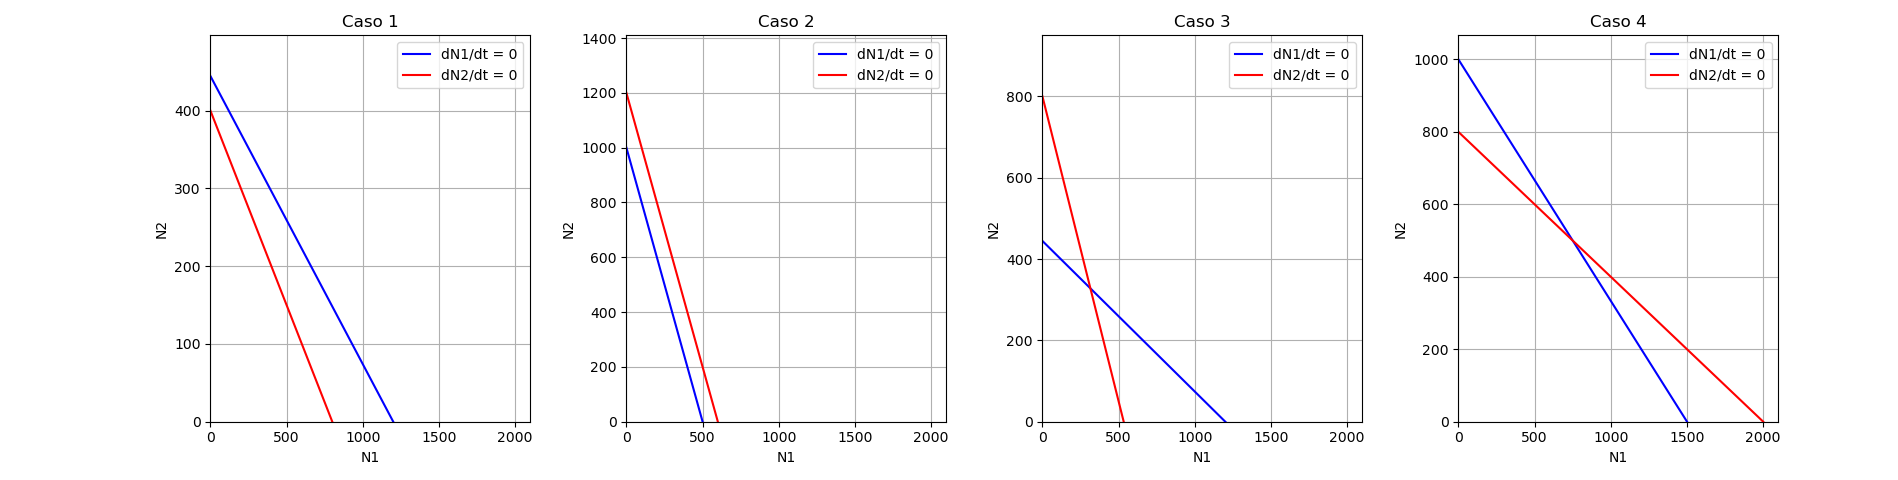
\includegraphics[width=1.3\textwidth]{tipos_de_isoclinas.png}}
        \caption{Ejemplos de isoclinas para cada uno de los casos.}
    \label{fig:isoclinas}
\end{figure*}

Observar de las ecuaciones (\ref{eq:(3)}) y (\ref{eq:(4)}) la tasa intrínseca de crecimiento \(r_i\) no está presente en las ecuaciones que definen a las isoclinas. Pero, si nos interesa representar la evolución temporal de las especies mediante series temporales dichos parámetros son necesarios, así como establecer \(N_1(t = 0)\) y \(N_2(t = 0)\) condiciones iniciales del sistema. Nos interesa observar la dinámica para \(r_i > 0\), \(r_i = 0\) y \(r_i < 0\) y como estos cambios afectan el desarrollo de la población de las demás especies. Aproximamos \(N_1(t)\) y \(N_2(t)\) a lo largo de un intervalo de tiempo \(t \epsilon [0, 100]\) utilizando el valor de \(h = ??\) encontrado en el el primer experimento de manera de minimizar el error cometido.

%   IMPORTANTE: ACÁ VAN LOS GRÁFICOS DE LA SERIE TEMPORAL VARIANDO r_1

Además, hay distintas condiciones iniciales para la población\footnote{Observar que \(N_1(t)\) y \(N_2(t)\) representan la población de cada especie en el tiempo \(t\) es por esto que toman valores no negativos.} de cada especie \(N_1(t = 0)\) y \(N_2(t = 0)\) que definen casos relativos a los valores de \(K_1\) y \(K_2\), representativos de la capacidad máxima de cada una de las especies que puede albergar el ecosistema. Entonces, El caso trivial sucede cuando la condición inicial es igual a 0, en este caso no hay población. Por otro lado, la población puede iniciar en una cantidad entre 0 y su respectivo \(K_i\). El último caso considera la posibilidad de que, a causa de algún tipo de intervención, la población inicial supera a la capacidad máxima del ambiente. 

% IMPORTANTE: ACÁ VAN LOS GRÁFICOS DE LA SERIE TEMPORAL VARIANDO N_1(0)

% IMPORTANTE: ACÁ HAY QUE PONER LA SERIE TEMPORAL PARA LOS DISTINTOS TIPOS DE ISOCLINAS CON UN R Y UN N INICIAL 

\end{document}